\subsection{Anden ordens butterworth filter}
\begin{figure}[H]
	\centering
	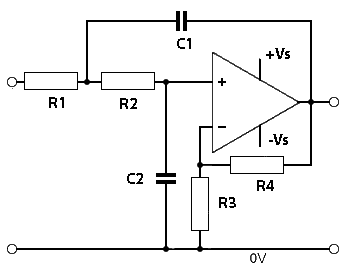
\includegraphics[width = 0.5\textwidth]{billeder/2ordensButterworth.png}
	\caption{2. ordens butterworth filter}\label{fig:butterworth}
\end{figure}
Normaliseriet polynomie som producerer et anden ordens butterwoth respons \fixme{Kilde: the analysis \& design of linear circuits – side 755}
\begin{equation}
	s^2 + 1.414s +1 = 0 
\end{equation}

\begin{equation}
	\zeta = \frac{1.414}{2} = 0.707
\end{equation}

Der bruges en anden metode til at bestemme R og $C_1$ og $C_2$. Det bestemmes at $R = 100k \Omega $, for at mindske spændingsdelingen mellem kredsløbet og spændingskilden.

Den ønskede knækfrekvens er $f_c = 11Hz$ og efter som $f_c = \frac{\omega_c}{2 \pi} $ så er $\omega_c = f_c * 2 * \pi = 22 \pi $

Nu løses de to ligninger med de to ubekendte $R \sqrt{C_1 * C_2} = \frac{1}{\omega_0}$ og $ \frac{C_2}{C_1} = \zeta^2$ og $C_1$ og $C_2$ bliver:

$C_1 = 2.046*10^-7F$ eller $ C_1 = -2.046*10^-7F$ \\
$C_2 = 1.023*10^-7F$ eller $ C_2 = -1.023*10^-7F$ \\

\subsection{Høj pas filter}
\begin{figure}[H]
	\centering
	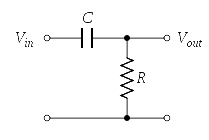
\includegraphics[width = 0.5\textwidth]{billeder/HighPass.png}
	\caption{1. ordens høj pas filter}\label{fig:highpass}
\end{figure}

Knæk frekvens $f_c = 0.3$ \\
Modstand værdi, $R = 1M\Omega$

Nu udregnes værdien af kondensatoren ved at isolere C: 
\begin{equation}
	f_c = \frac{1}{2\pi * R * C} \Rightarrow C = 5.3052 * 10^-7F
\end{equation}


Dette bliver en kondensator på 530nF, den nærmeste komponent hedder 680nF og derfor udregnes den nye knæk frekvens til: 
\begin{equation}
	f_c = \frac{1}{2\pi * R * 680 * 10^-9} = 0.23Hz
\end{equation}



\subsection{Lav pas filter}
\begin{figure}[H]
	\centering
	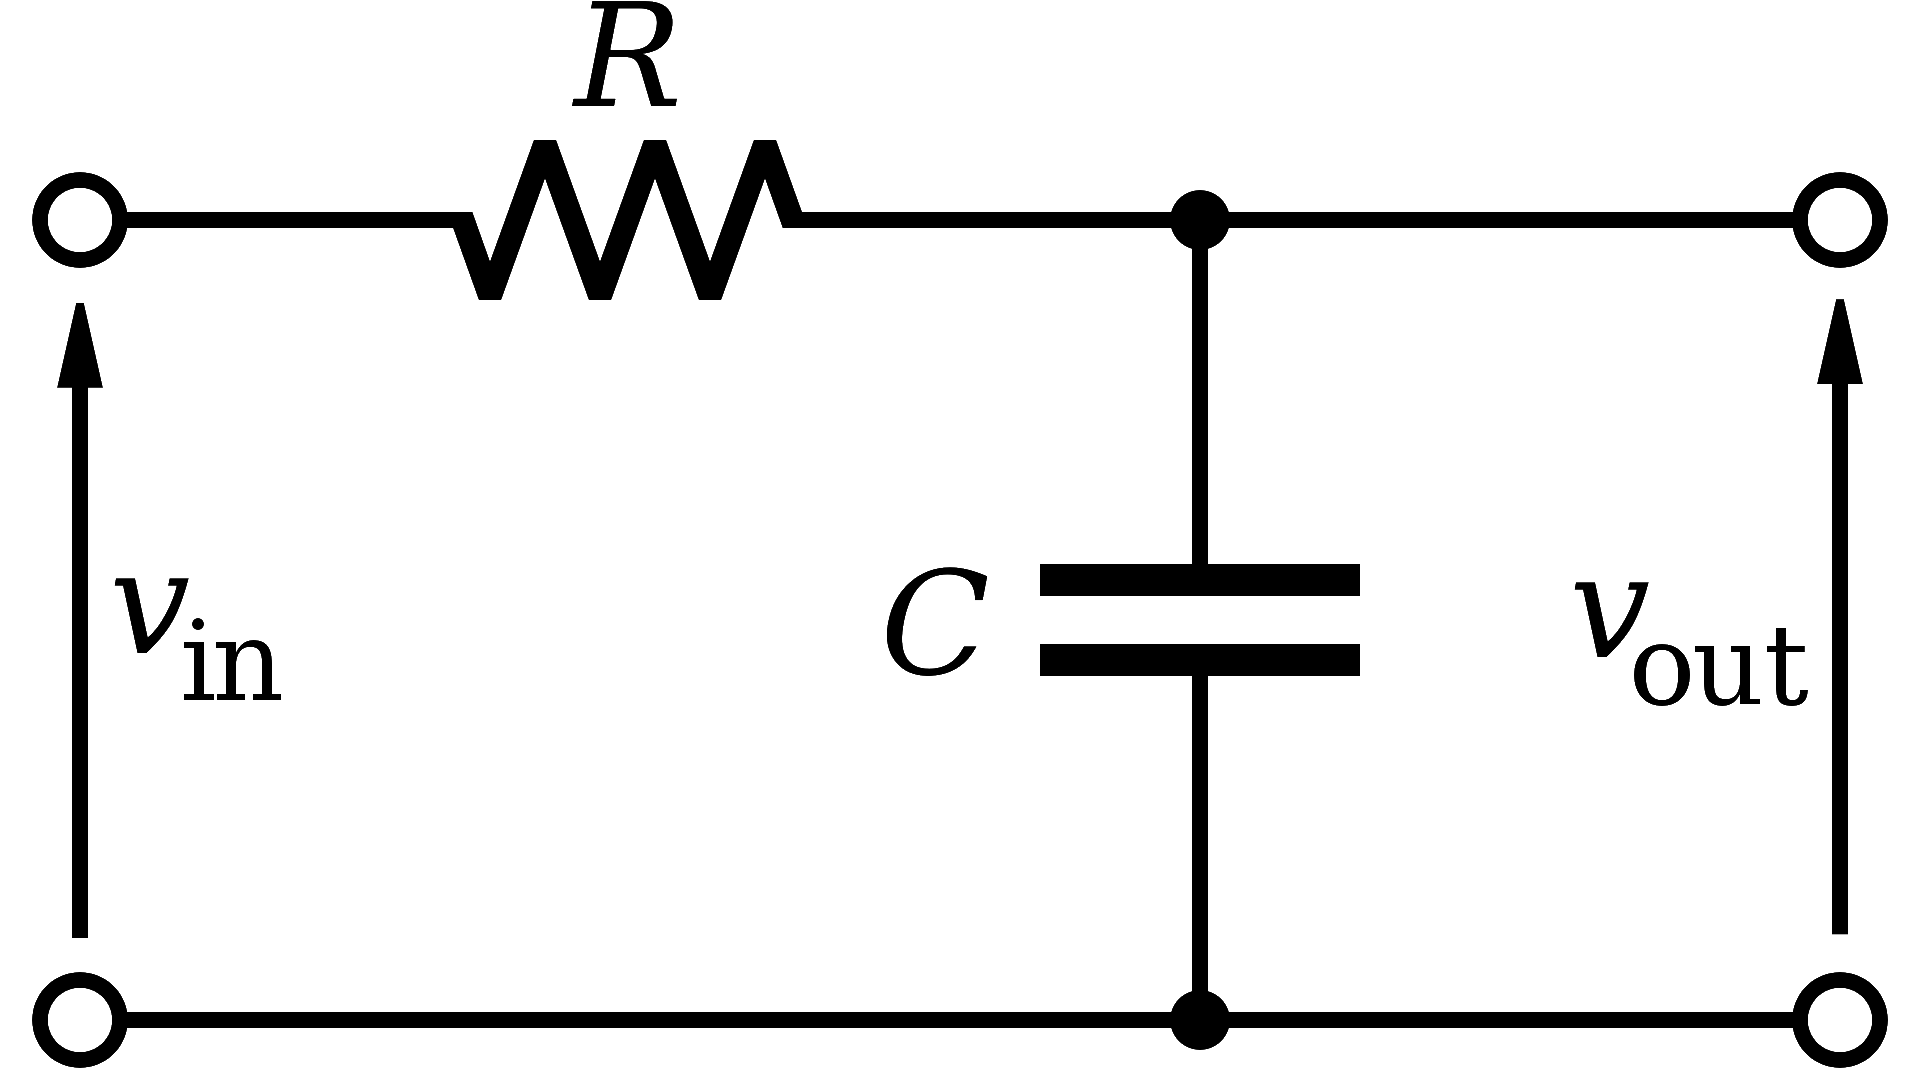
\includegraphics[width = 0.5\textwidth]{billeder/LowPass.png}
	\caption{1. ordens lav pas filter}\label{fig:lowpass}
\end{figure}
Knæk frekvens $f_c = 0.3$ \\
Modstand værdi, $R = 1M\Omega$

Nu udregnes værdien af kondensatoren ved at isolere C:
\begin{equation}
	f_c = \frac{1}{2\pi * R * C} \Rightarrow C = 5.3052 * 10^-7F
\end{equation}


Dette bliver en kondensator på 530nF, den nærmeste komponent hedder 680nF og derfor udregnes den nye knæk frekvens til:
\begin{equation}
	 f_c = \frac{1}{2\pi * R * 680 * 10^-9} = 0.23Hz
\end{equation}


\newpage
\subsection{Gain på manchet oscillationer }
\begin{figure}[H]
	\centering
	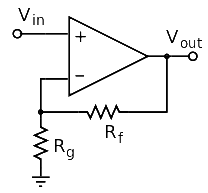
\includegraphics[width = 0.5\textwidth]{billeder/OpAMP_gain.png}
	\caption{Gain til manchet oscillationer}\label{fig:opam1}
\end{figure}
\textbf{Udregning af gain: } \\
Der ønskes et gain på 2, dvs $A = 100$
\begin{equation}
	A = \frac{V_0}{V_i} = 1 + \frac{R_f}{R_g}
\end{equation}


\textbf{Udregning af komponenter:}\\
Indsættelse af komponent værdier, $R_f$ sættes til $100k\Omega$ og $R_g$ udregnes: 
\begin{equation}
	 A = 1 + \frac{R_f}{R_g} \Rightarrow R_g =  1010
\end{equation}

Derfor vælges $R_g$ til at være $1k\Omega$

\subsection{Gain på manchettryk signal }
\begin{figure}[H]
	\centering
	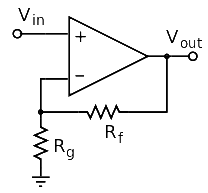
\includegraphics[width = 0.5\textwidth]{billeder/OpAMP_gain.png}
	\caption{Gain til manchettryk signal}\label{fig:opam2}
\end{figure}
\textbf{Udregning af gain: } \\
Der ønskes et gain på 100, dvs $A = 2$
\begin{equation}
	A = \frac{V_0}{V_i} = 1 + \frac{R_f}{R_g}
\end{equation}

\textbf{Udregning af komponenter:}\\
Indsættelse af komponent værdier, $R_f$ sættes til $100k\Omega$ og $R_g$ udregnes:
\begin{equation}
	 A = 1 + \frac{R_f}{R_g} \Rightarrow R_g = 100000
\end{equation}

Derfor vælges $R_g$ til at være $100k\Omega$